\documentclass{beamer}
\usetheme[deutsch]{KIT}

%\usepackage{etex}
\usepackage[utf8]{inputenc}
\usepackage[T1]{fontenc}
\usepackage{babel}
\usepackage{tikz,calc,ifthen}
\usepackage{mathtools}
\usepackage[normalem]{ulem}
\usepackage{graphicx}
\usepackage{listings, caption}
\usepackage{color}
\usepackage{colortbl}
\usepackage{textcomp}
\usepackage{eurosym} % used for \euro
%\usepackage{pgfplots}
%\usepgfplotslibrary{statistics}
\usetikzlibrary{positioning,calc,arrows,shapes}
\tikzset{
  every node/.style={transform shape},
  auto,
  block/.style={align=center,rectangle,draw,minimum height=20pt,minimum width=30pt},
  >=triangle 60,
  alt/.code args={<#1>#2#3}{%
      \alt<#1>{\pgfkeysalso{#2}}{\pgfkeysalso{#3}}
  },
  beameralert/.style={alt=<#1>{color=green!80!black}{}},
  mythick/.style={line width=1.4pt}
}

\newcommand*{\maxwidthofm}[2]{\maxof{\widthof{$#1$}}{\widthof{$#2$}}}
\newcommand<>*{\robustaltm}[2]{
  \alt#3
  {\mathmakebox[\maxwidthofm{#1}{#2}]{#1}\vphantom{#1#2}}
    {\mathmakebox[\maxwidthofm{#1}{#2}]{#2}\vphantom{#1#2}}
}

\newcommand<>*{\nodealert}[1]{\only#2{\draw[overlay,mythick,color=green!80!black] (#1.north west) rectangle (#1.south east)}}

\title{Projekt 1 -- Jacobi- und Gauß-Seidel-Verfahren}
\author{Sarah Lutteropp und Johannes Sailer}
\subtitle{\insertauthor}
\institute[Lehrstuhl für Rechnerarchitektur und Parallelverarbeitung]{Lehrstuhl für Rechnerarchitektur und Parallelverarbeitung}
\date{17.02.2016}
\KITtitleimage{images/28740_the_matrix_matrix_code.jpg}

\begin{document}

\begin{frame}
    \maketitle
\end{frame}

\begin{frame}
   \frametitle{Gliederung}
   \tableofcontents
 \end{frame}

\section{Aufgabenstellung}

\begin{frame}
\frametitle{Aufgabenstellung}
\begin{block}{Approximation von Stoffkonzentrationen}
\begin{align}
-\Delta u(x,y) &= f(x,y) \quad \forall (x,y) \in (0,1)^2\\
u(x,y) &= 0 \qquad \text{~~~~~} \forall (x,y) \in [0,1]^2 \backslash (0,1)^2
\end{align}

$$\Delta u = \frac{\partial^2 u}{\partial x^2} + \frac{\partial^2 u}{\partial y^2}$$
\end{block}
\end{frame}

\begin{frame}
\frametitle{Approximation von Stoffkonzentrationen}
\begin{center}
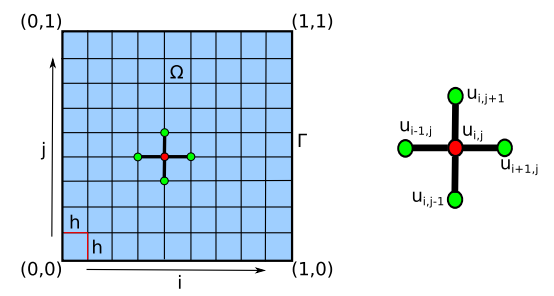
\includegraphics[scale=0.5]{images/aufgabenstellung.png}
\\Approximation mit Methode der Finiten Differenzen
\end{center}
$$-u_{i,j-1} - u_{i-1,j} + 4 u_{i,j} - u_{i,j+1} - u_{i+1,j} = h^2 f(x_i, y_j)$$
\end{frame}

\begin{frame}
\frametitle{Konkretes Beispiel}
\begin{block}{Für $h=\frac{1}{3}$}
\begin{center}
\vspace{-0.8cm}
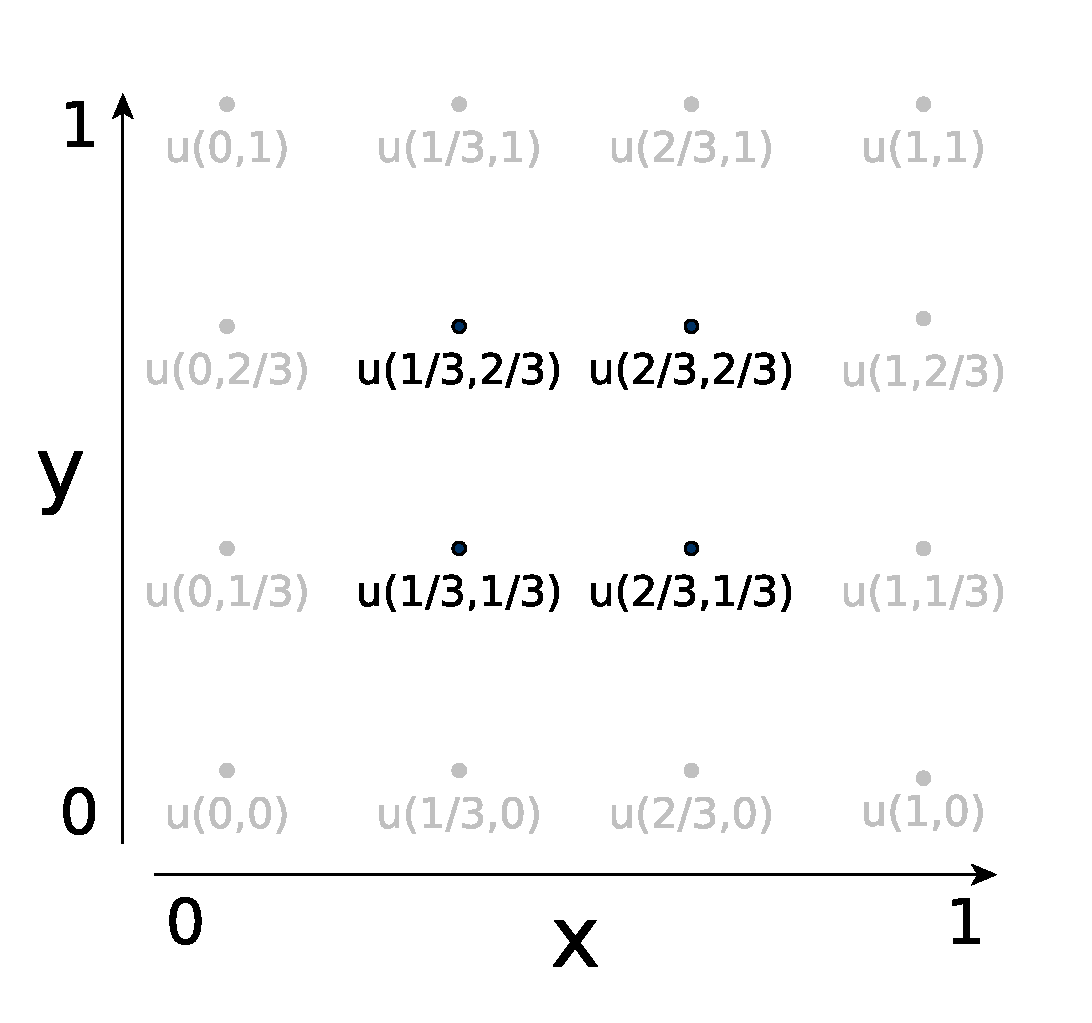
\includegraphics[scale=0.4]{images/h_1_drittel.pdf}
\end{center}
\end{block}
\end{frame}

\begin{frame}
\frametitle{Konkretes Beispiel}
\begin{block}{Für $h=\frac{1}{3}$}
\begin{center}
\vspace{-0.8cm}
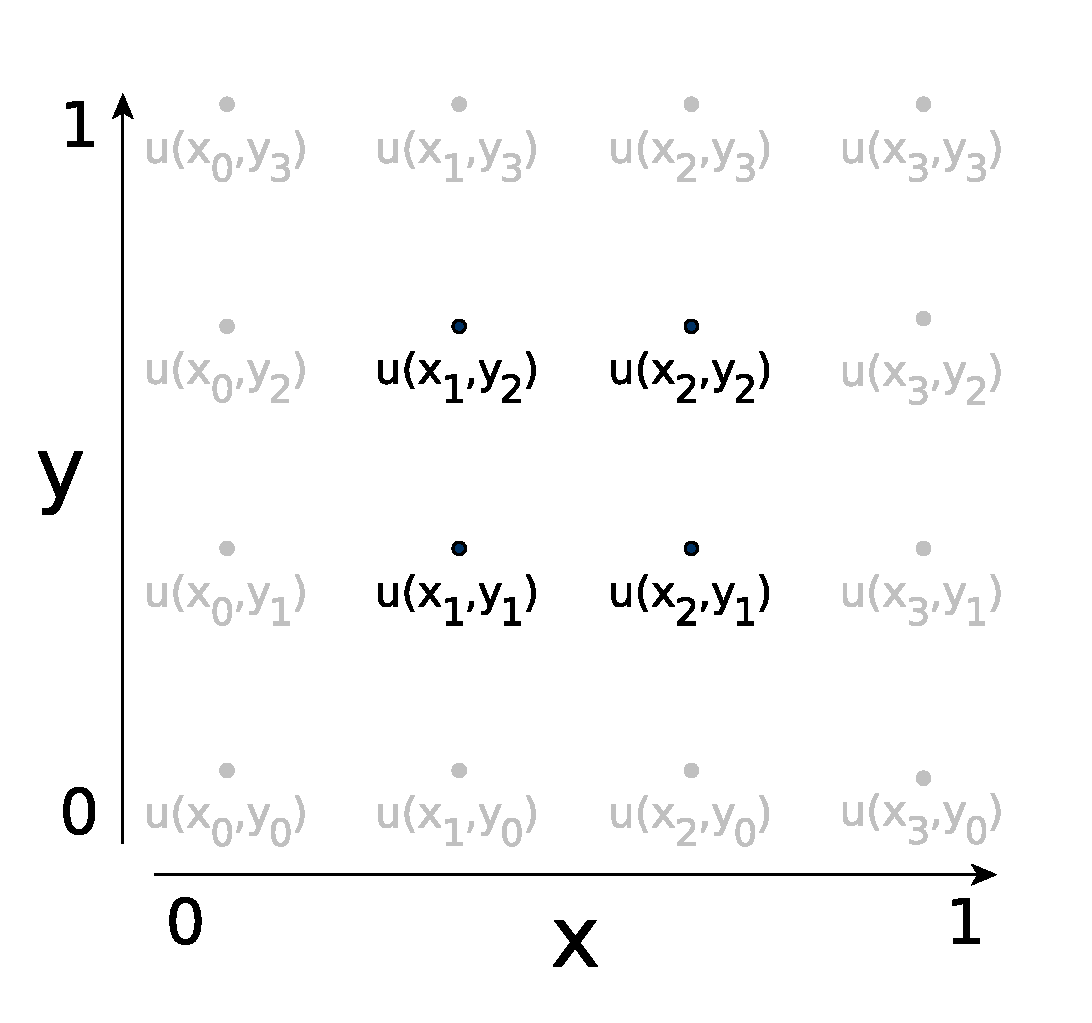
\includegraphics[scale=0.4]{images/h_1_drittel_x.pdf}
\end{center}
\end{block}
\end{frame}

\begin{frame}
\frametitle{Konkretes Beispiel}
\begin{block}{Für $h=\frac{1}{3}$}
\begin{center}
\vspace{-0.8cm}
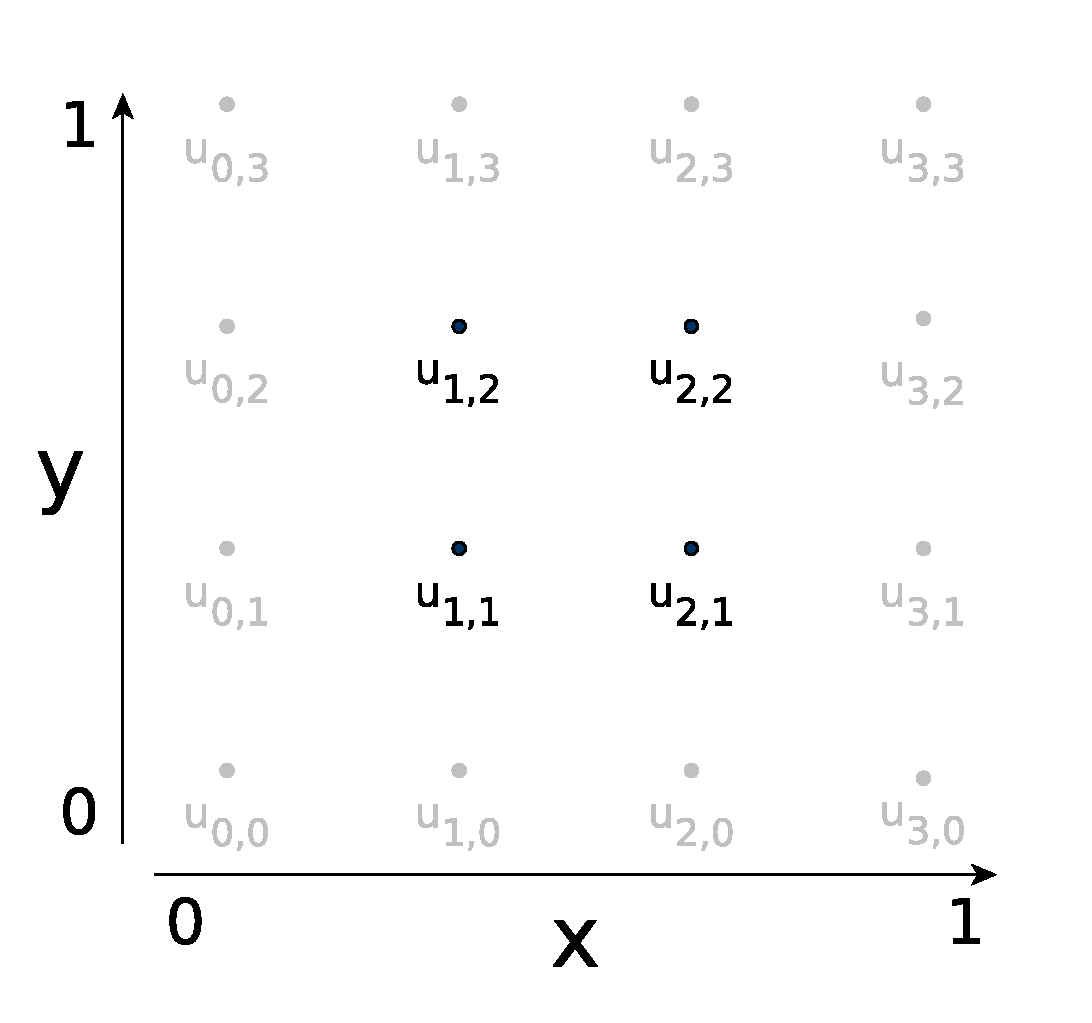
\includegraphics[scale=0.4]{images/h_1_drittel_zahl.pdf}
\end{center}
\end{block}
\end{frame}

\begin{frame}
\frametitle{Konkretes Beispiel}
\begin{block}{Für $h=\frac{1}{3}$}

\vspace{-1cm}

\begin{center}
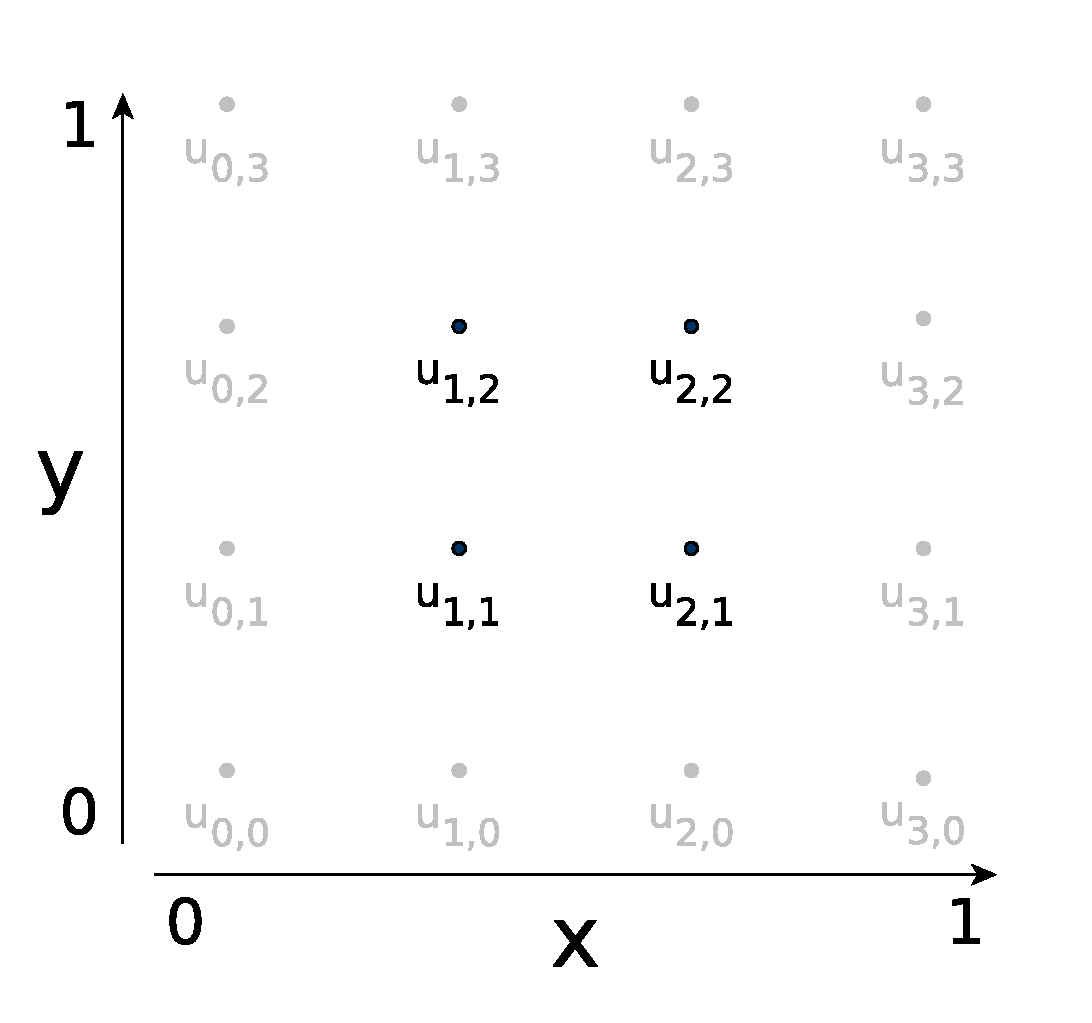
\includegraphics[scale=0.2]{images/h_1_drittel_zahl.pdf}
\end{center}

\vspace{-1cm}

$$-u_{i,j-1} - u_{i-1,j} + 4 u_{i,j} - u_{i,j+1} - u_{i+1,j} = h^2 f(x_i, y_j)$$

$$\begin{pmatrix}
4 & -1 & -1 & 0 \\ 
-1 & 4 & 0 & -1 \\ 
-1 & 0 & 4 & -1 \\ 
0 & -1 & -1 & 4
\end{pmatrix} *
\begin{pmatrix}
u_{1,1} \\ 
u_{1,2} \\ 
u_{2,1} \\ 
u_{2,2}
\end{pmatrix} = \left(\frac{1}{3}\right)^2 *
\begin{pmatrix}
f(1/3,1/3) \\ 
f(1/3,2/3) \\ 
f(2/3,1/3) \\ 
f(2/3,2/3)
\end{pmatrix}
$$
\end{block}
$\Rightarrow$ Löse $Au=b$
\end{frame}

\section{Mathematischer Hintergrund}

\subsection*{Herleitung der Verfahren}

\begin{frame}
\frametitle{Herleitung der Verfahren}
\begin{center}
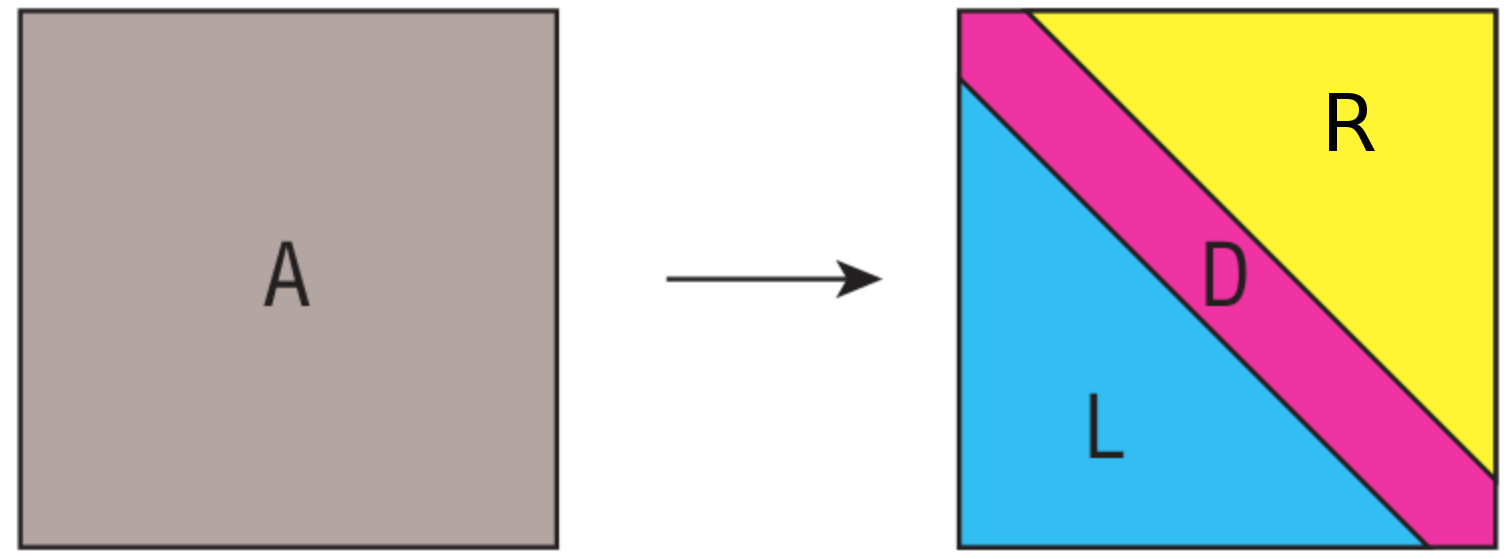
\includegraphics[scale=0.1]{images/zerlegung_A.png}
\end{center}

$$Au = b$$
$$\Leftrightarrow (D+L+R)u = b \Leftrightarrow \ldots$$

\begin{itemize}
\item Jacobi-Verfahren: \qquad \quad $u^{(k)} = D^{-1}  \left(b -(L+R)  u^{(k-1)}\right)$
\item Gauß-Seidel-Verfahren: ~$u^{(k)} = D^{-1} \left(b - Lu^{(k)} - Ru^{(k-1)}\right)$
\end{itemize}

\end{frame}

\begin{frame}
\frametitle{Herleitung der Verfahren}
\begin{center}
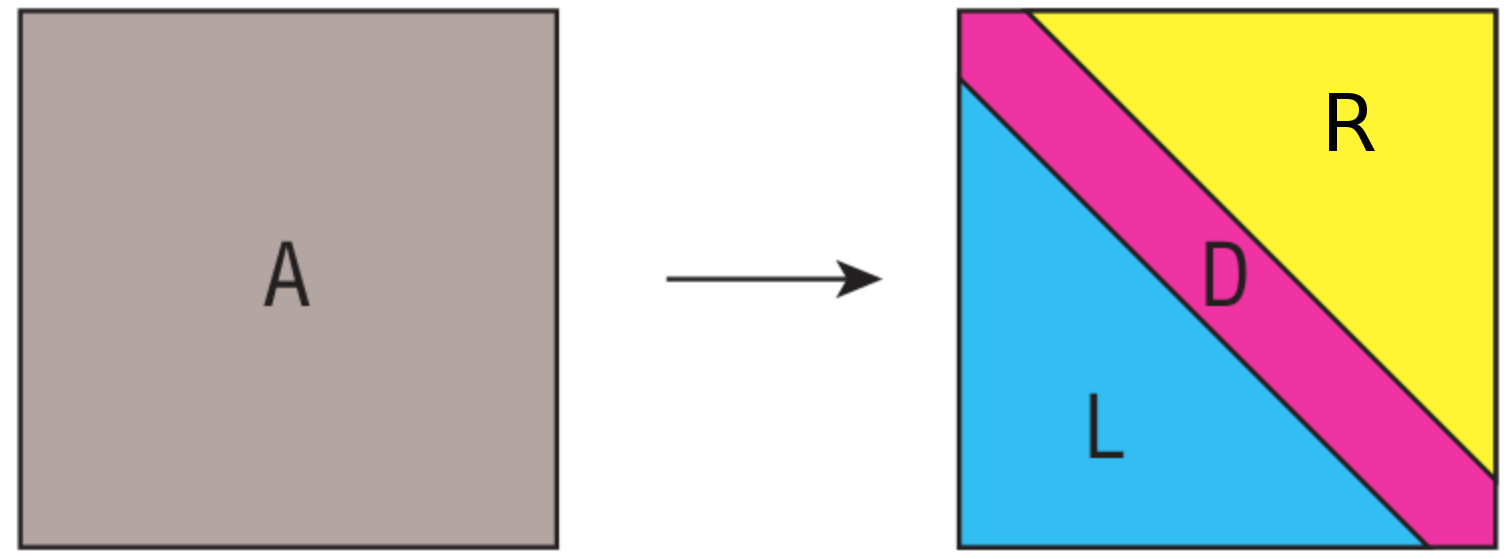
\includegraphics[scale=0.1]{images/zerlegung_A.png}
\end{center}

\begin{itemize}
\item Jacobi-Verfahren: $$u_i^{(k)} = \frac{1}{a_{ii}} * \left(b_i - \sum_{j \neq i}{a_{ij} u_j^{(k-1)}}\right) \quad \forall i = 1, \ldots, n^2$$
\item Gauß-Seidel-Verfahren: $$u_i^{(k)} = \frac{1}{a_{ii}} * \left(b_i - \sum_{j=1}^{i-1}{a_{ij} u_j^{(k)}} - \sum_{j=i+1}^{n^2}{a_{ij}*u_j^{(k-1)}}\right) \quad \forall i = 1, \ldots, n^2$$
\end{itemize}

\end{frame}

\begin{frame}
\frametitle{Unsere Lösungsmatrix $U$}
\begin{block}{Für $h=\frac{1}{3}$}

Betrachte statt 

$$u = \begin{pmatrix}
u_{1,1} \\ 
u_{1,2} \\ 
u_{2,1} \\ 
u_{2,2}
\end{pmatrix} \qquad
U=
\begin{tabular}{|c|c|c|c|}
\hline 
\cellcolor[gray]{0.8}$u_{0,0}$ & \cellcolor[gray]{0.8}$u_{1,0}$ & \cellcolor[gray]{0.8}$u_{2,0}$ & \cellcolor[gray]{0.8}$u_{3,0}$ \\ 
\hline 
\cellcolor[gray]{0.8}$u_{0,1}$ & $u_{1,1}$ & $u_{2,1}$ & \cellcolor[gray]{0.8}$u_{3,1}$ \\ 
\hline 
\cellcolor[gray]{0.8}$u_{0,2}$ & $u_{1,2}$ & $u_{2,2}$ & \cellcolor[gray]{0.8}$u_{3,2}$ \\ 
\hline 
\cellcolor[gray]{0.8}$u_{0,3}$ & \cellcolor[gray]{0.8}$u_{1,3}$ & \cellcolor[gray]{0.8}$u_{2,3}$ & \cellcolor[gray]{0.8}$u_{3,3}$ \\ 
\hline 
\end{tabular} 
$$

(Die Randeinträge sind hierbei $0$)
\end{block}

\begin{block}{Vorteil}
\begin{itemize}
\item Jeder Eintrag in $U$ entspricht einem Punkt im Gitter
\item Parallelisierung intuitiver
\end{itemize}
\end{block}

\end{frame}

\subsection*{Abbruchkriterium}

\begin{frame}
\frametitle{Unser Abbruchkriterium}
\begin{huge}
$$\frac{\sum_{i,j} {| u_{i,j}^{(k)} - u_{i,j}^{(k-1)} |}}{size * size} \leq \texttt{TOL}$$
\end{huge}

\begin{columns}[c]
		\column[c]{5cm}
		\vspace{0.6cm}
		\begin{block}{Vorteile}
\begin{itemize}
	\item Sprunglos
	\item Implementierung mit \texttt{\#pragma omp reduce}
\end{itemize}
\end{block}
		\column{5cm}
		\begin{block}{Nachteile}
\begin{itemize}
\item Maximum der Differenzen wäre exakter
\end{itemize}
\end{block}
	\end{columns}
\end{frame}

\begin{frame}
\frametitle{Unser Abbruchkriterium}
\begin{center}
Beide Verfahren konvergieren.
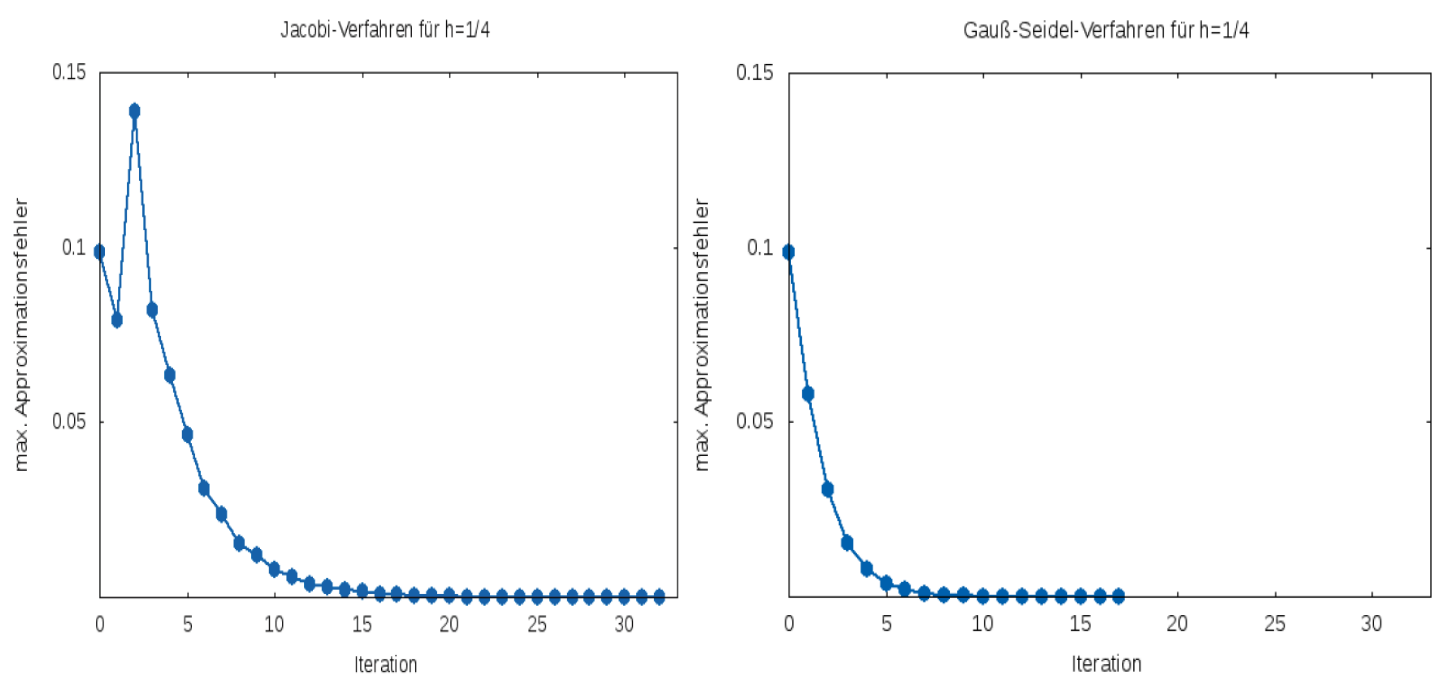
\includegraphics[scale=0.232]{images/konvergenz.png}
\end{center}
\end{frame}

\section{Parallelisierung}

\begin{frame}
\frametitle{Parallele Ansätze -- Jacobi-Verfahren}
Keine Abhängigkeiten innerhalb einer Iteration
\begin{center}
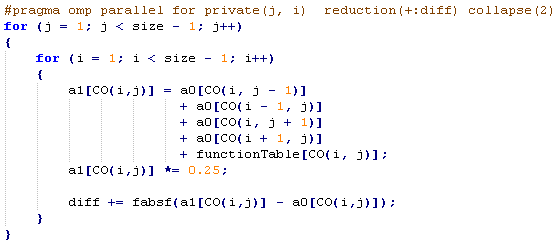
\includegraphics[scale=0.75]{images/code_jacobi.png}
\end{center}
\end{frame}

\begin{frame}
\frametitle{Parallele Ansätze -- Jacobi-Verfahren}
\begin{block}{Zusätzliche Optimierung: SSE-Vektorinstruktionen}
\begin{center}
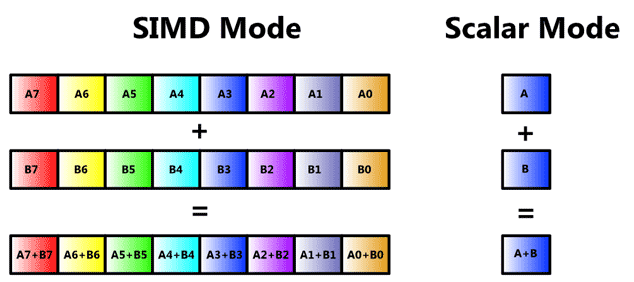
\includegraphics[scale=0.4]{images/simd.png}
\end{center}
\end{block}
\end{frame}

\begin{frame}
\frametitle{Parallele Ansätze -- Gauß-Seidel-Wavefront}
\begin{itemize}
\item Abhängigkeiten innerhalb einer Iteration:
$$u_{i,j}^{(k+1)} = \frac{1}{4} u_{i,j-1}^{(k+1)} + u_{i-1,j}^{(k+1)} + u_{i,j+1}^{(k)} + u_{i+1,j}^{(k)} + h^2 f(x_i, y_j)$$
\item 1. Möglichkeit: Wavefront
\begin{center}
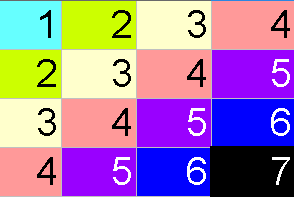
\includegraphics[scale=0.7]{images/wavefront.png}
\end{center}
\end{itemize}
\end{frame}

\begin{frame}
\frametitle{Parallele Ansätze -- Gauß-Seidel-Wavefront}

\begin{block}{Nachteile Wavefront}
\begin{itemize}
	\item Schlecht für Cache
	\begin{center}
	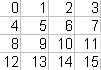
\includegraphics[scale=0.8]{images/cache_1.png} \qquad
	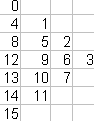
\includegraphics[scale=0.8]{images/cache_2.png}
	\end{center}
	\item Aufwändige Berechnung der Indizes
	\item Geringe Parallelität bei kleinen Diagonalen
	\item Allgemein großer Overhead
\end{itemize}
\end{block}

\end{frame}

\begin{frame}
\frametitle{Parallele Ansätze -- Gauß-Seidel-RotSchwarz}
\begin{block}{Zweite Möglichkeit: Rot-Schwarz-Iteration}
	Färben der Matrixeinträge nach folgendem Schema:
	\begin{center}
	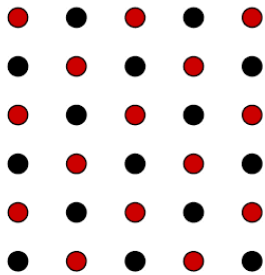
\includegraphics[scale=0.4]{images/rotschwarz_faerbung.png}
	\end{center}
	\begin{enumerate}
	\item Berechnen aller roten Einträge
	\item Berechnen aller schwarzen Einträge
	\end{enumerate}
\end{block}
\end{frame}

\begin{frame}
\frametitle{Parallele Ansätze -- Gauß-Seidel-RotSchwarz}
\begin{block}{Optimierung: Rot-Matrix und Schwarz-Matrix separat}
\begin{itemize}
\item Cache-Effizienz
\item Sehr einfache Berechnung der Indizes
\item Beschleunigung mit SSE-Vektorinstruktionen
\end{itemize}
\end{block}
\begin{center}
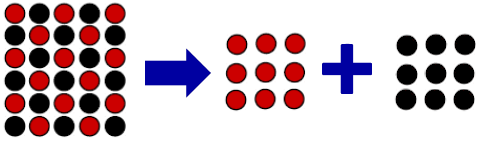
\includegraphics[scale=0.5]{images/splitting.png}
\end{center}
\end{frame}

\begin{frame}
\frametitle{Parallele Ansätze -- Gauß-Seidel-RotSchwarz}
\begin{block}{Berechnung der Indizes, $size$ ungerade für $size=7$}
\begin{center}
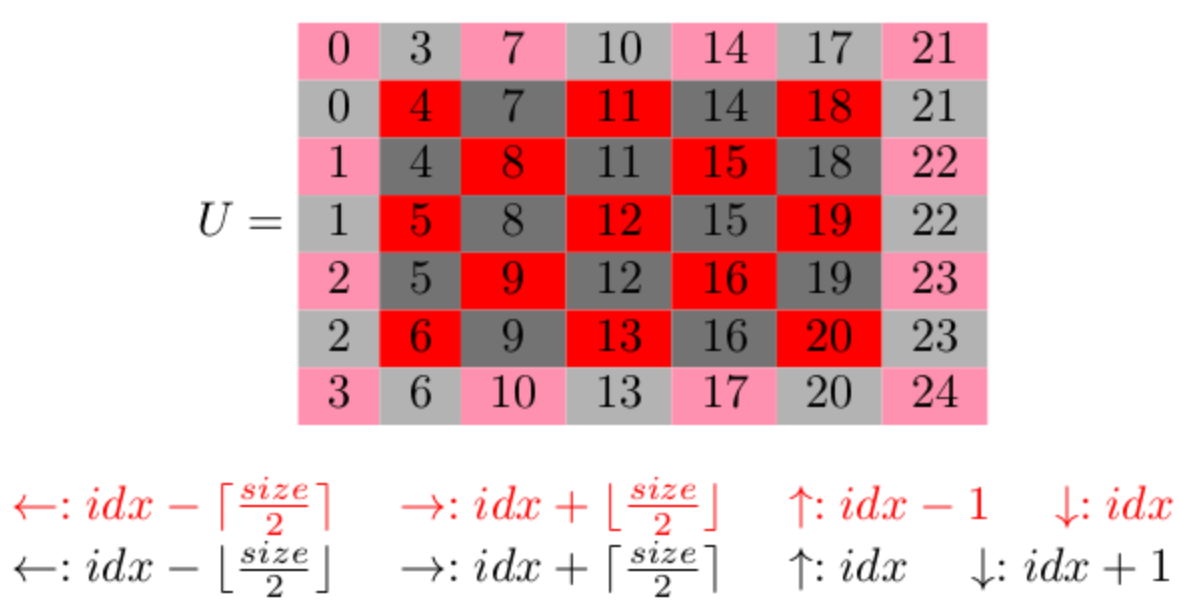
\includegraphics[scale=0.2]{images/indizes_ungerade.png}
\end{center}
\end{block}
\end{frame}

\begin{frame}
\frametitle{Parallele Ansätze -- Gauß-Seidel-RotSchwarz}
\begin{block}{Berechnung der Indizes, $size$ gerade für $size=6$}
\begin{center}
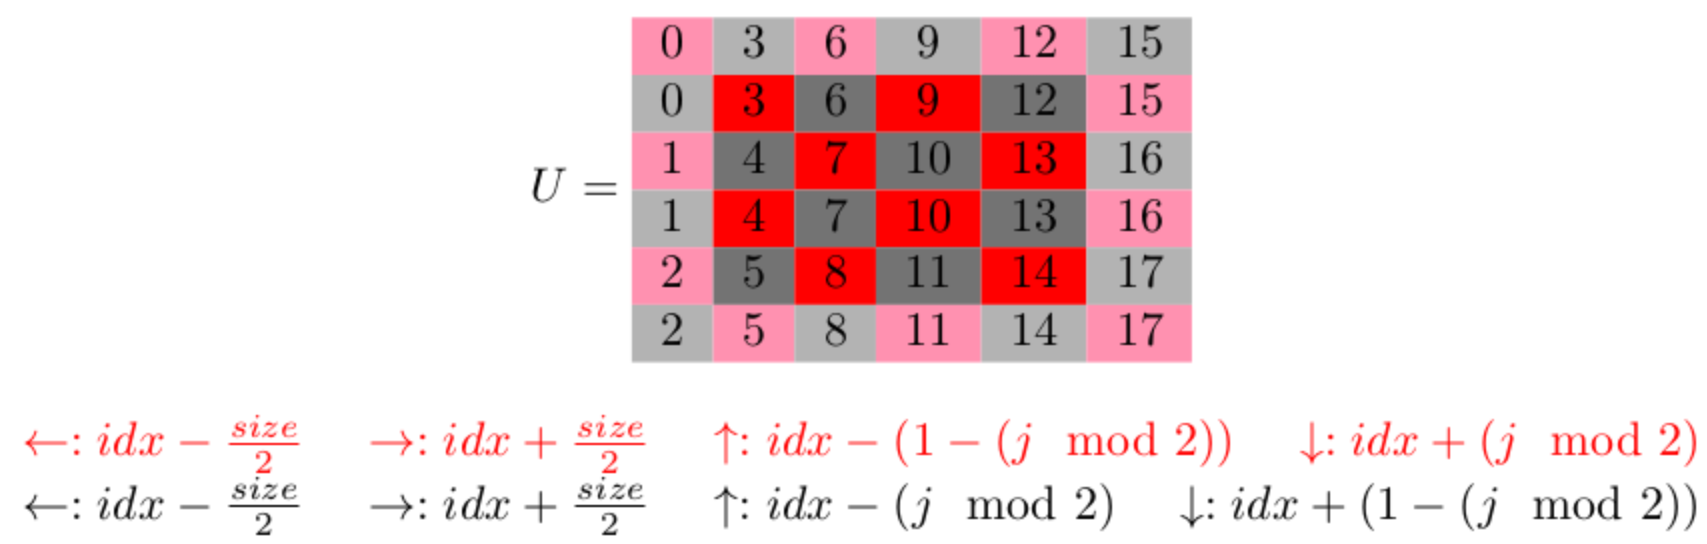
\includegraphics[scale=0.2]{images/indizes_gerade.png}
\end{center}
Loop-Unrolling vermeidet Modulo-Operation!
\end{block}
\end{frame}


\section{Experimentelle Auswertung}

\begin{frame}
\frametitle{Auswertung ohne Abbruchkriterium}
\begin{center}
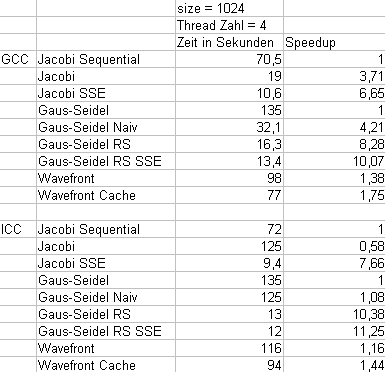
\includegraphics[scale=0.65]{images/tabelle_auswertung_ohne.png}
\end{center}
\end{frame}

\begin{frame}
\frametitle{Auswertung mit Abbruchkriterium}
\begin{center}
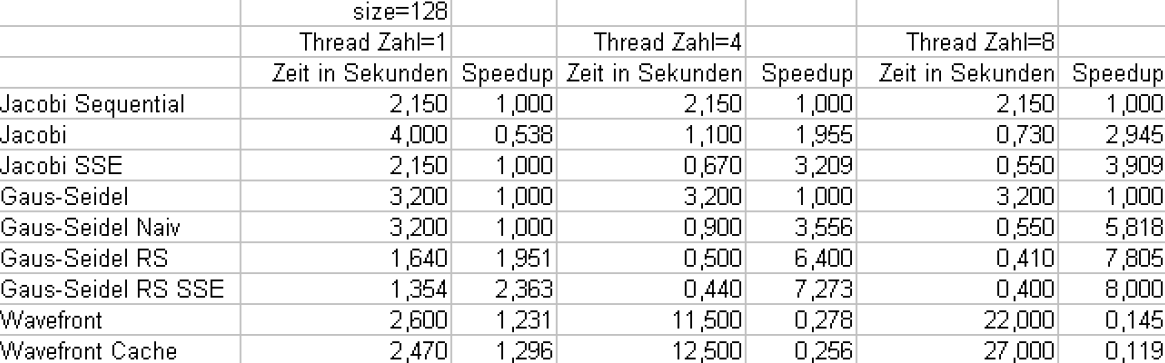
\includegraphics[scale=0.35]{images/tabelle_auswertung_mit.png}
\end{center}
\end{frame}

\begin{frame}
\frametitle{Auswertung mit Abbruchkriterium}
\begin{center}
\vspace{-0.7cm}
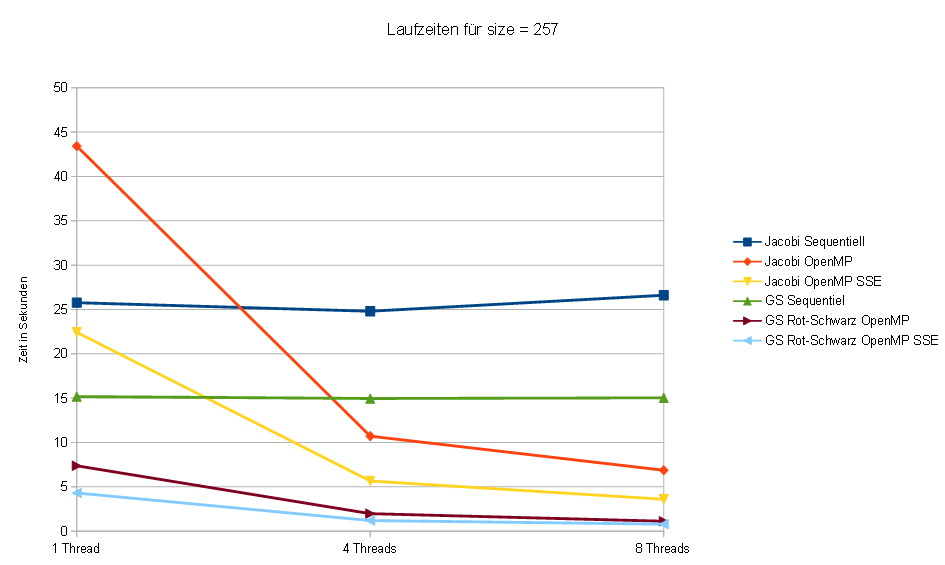
\includegraphics[scale=0.47]{images/bild_auswertung_mit.png}
\end{center}
\end{frame}

\begin{frame}
\frametitle{Auswertung mit Abbruchkriterium}
\begin{center}
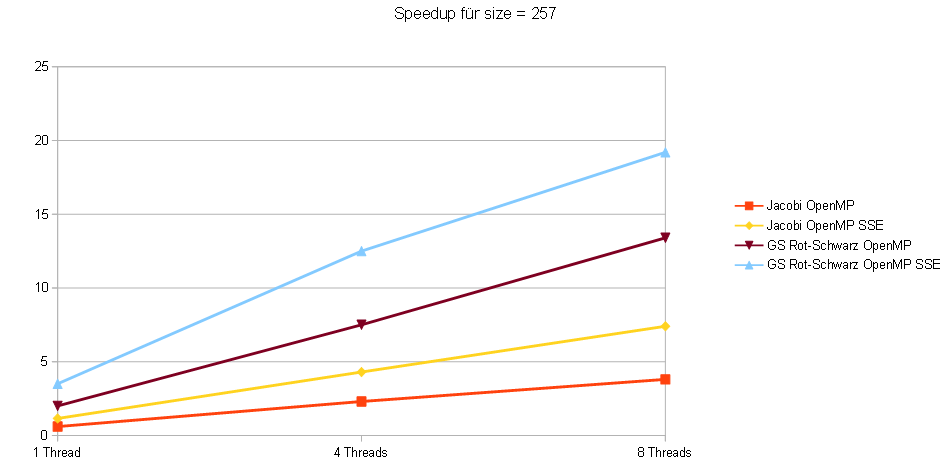
\includegraphics[scale=0.47]{images/bild_auswertung_ohne.png}
\end{center}
\end{frame}

\begin{frame}
\frametitle{Auswertung mit Abbruchkriterium}
\begin{center}
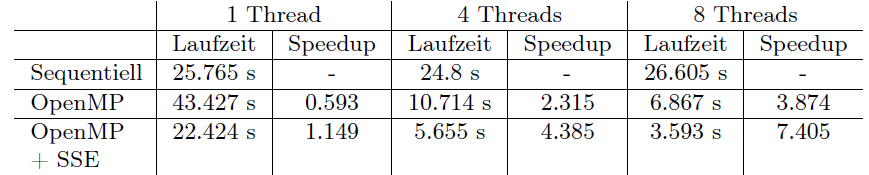
\includegraphics[scale=0.45]{images/tabelle_auswertung_ohne_2.png}\\
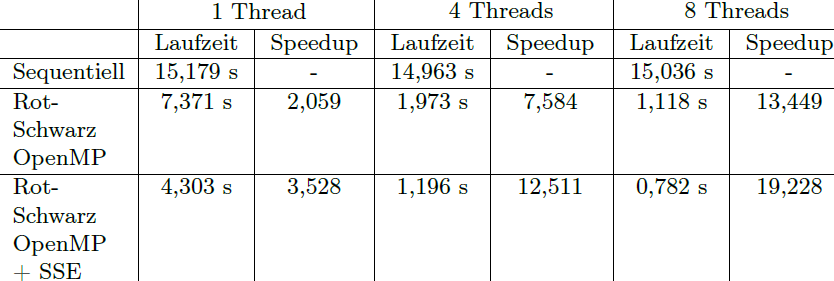
\includegraphics[scale=0.45]{images/tabelle_auswertung_ohne_3.png}
\end{center}
\end{frame}

\section{Fazit}

\begin{frame}
\frametitle{Fazit}
\begin{itemize}
\item Gauß-Seidel konvergiert doppelt so schnell
\item Rot-Schwarz-Iteration liefert den besten Speedup
\end{itemize}
\end{frame}

\end{document}


